\documentclass{article}
\usepackage[utf8]{inputenc}
\usepackage{amsmath}
\usepackage{amsfonts}
\usepackage{amssymb}
\usepackage{graphicx}
\usepackage{geometry}
\usepackage{xcolor}
\usepackage{gensymb}
\usepackage{hyperref}
\usepackage{gensymb}
\usepackage{listings}

\newcommand{\inv}{^{-1}}   
\newcommand{\Z}{\mathbb Z}
\newcommand{\R}{\mathbb R}
\newcommand{\Q}{\mathbb Q}
\newcommand{\C}{\mathbb C}
\newcommand{\N}{\mathbb N}

\begin{document}

\medskip\noindent\textbf{1.} 

    Here's my 12V power supply:
    \begin{center} 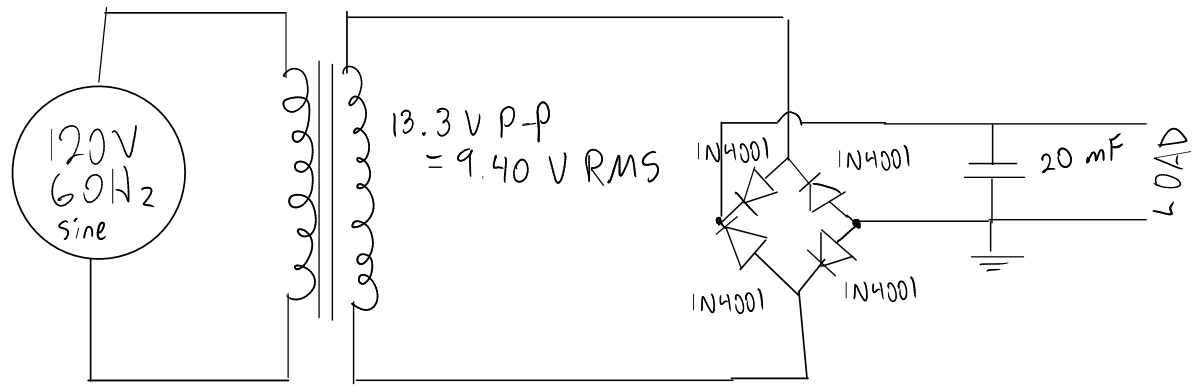
\includegraphics[scale=.3]{power_supply.png} \end{center}

    I solved for the capacitance using $V_{\text{ripple}} = \frac{I_{\text{out}}}{fC},$ and arrived at $C = \frac{1}{48} \approx 20$mF.

\medskip\noindent\textbf{2.} 

    Gain = $\frac{R_1 + R_2}{R_1} = \frac{64}{8} = 8.$

    The figure below shows $\text{V}_{\text{in}}$ in blue and $\text{V}_{\text{out}}$ in green.
    \begin{center}
        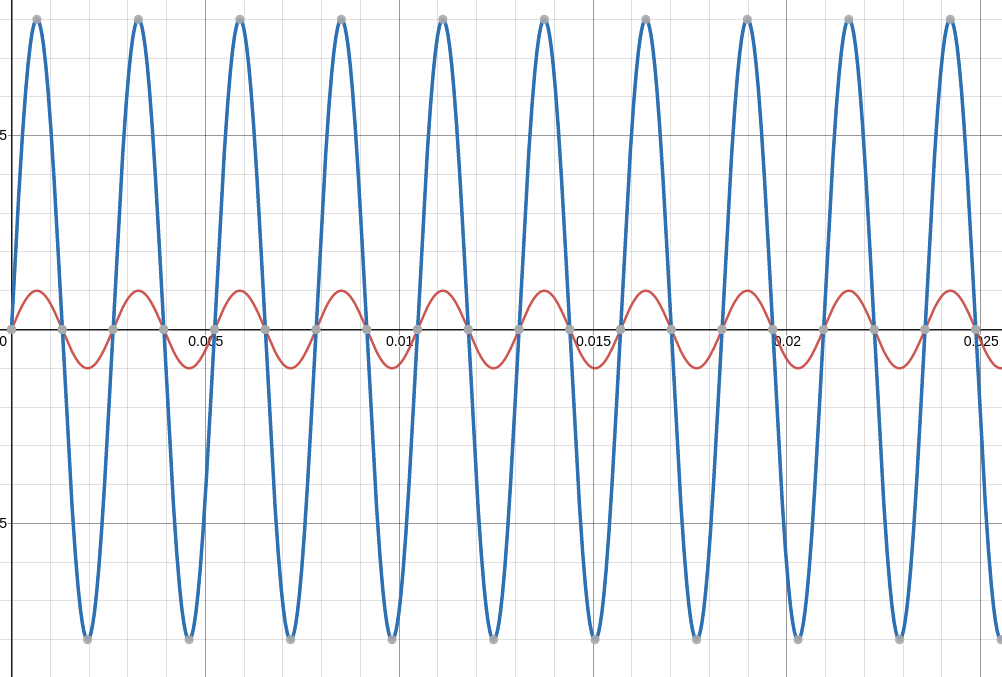
\includegraphics[scale=.5]{2.png}
    \end{center}

\newpage\noindent\textbf{3.}

    The negative input to the op-amp will ``want" to be at 0V.
    Thus, the current through the 42.2k$\Omega$ resistor will be $\frac{-15-0}{42200} \approx -.000355$A.
    Similarly, the current through the 9k$\Omega$ resistor will be $\frac{\text{V}_{\text{in}}}{9000}$A, and the current through the 5k$\Omega$ capacitor will be $\frac{\text{V}_{\text{out}}}{5000}$A.
    Because the op-amp inputs draw no current, we know that these currents must sum to 0.
    Then, we can solve to find that $$\text{V}_{\text{out}} = \frac{15.975-5\text{V}_{\text{in}}}{9}.$$

\medskip\noindent\textbf{4.}

\medskip\noindent\textbf{a)} The voltage at $a$ will be $20 \cdot \frac{3}{23} \approx 1.96$V

    The current through the 1k resistor will be $\frac{a}{1000}$, and the current through the 10k resistor will be $-\frac{\text{V}_{\text{out}}}{10000}$.
    These currents must be equal, so $a = -\frac{\text{V}_{\text{out}}}{10}$.
    By the same logic, the current through the 20k resistor is $\frac{15-a}{20000}$, and the current through the 3k resistor is $\frac{a}{3000}$.
    Again, the currents in and out of this node must be equal, so we can solve for $a$ to find $a = \frac{45}{83}$V.
    Thus, $\text{V}_{\text{out}} = -\frac{450}{83} \approx -5.42$V.

\medskip\noindent\textbf{5.}
    
    Because the inputs to an op-amp draw no current, the voltage at $a$ is not affected by the rest of the circuit.
    Thus, $\text{V}_{\text{out}}$ will be $-10$ times the voltage at $a$ from \textbf{a)} (so -19.6V).

\newpage\noindent\textbf{6.}

    \begin{center} 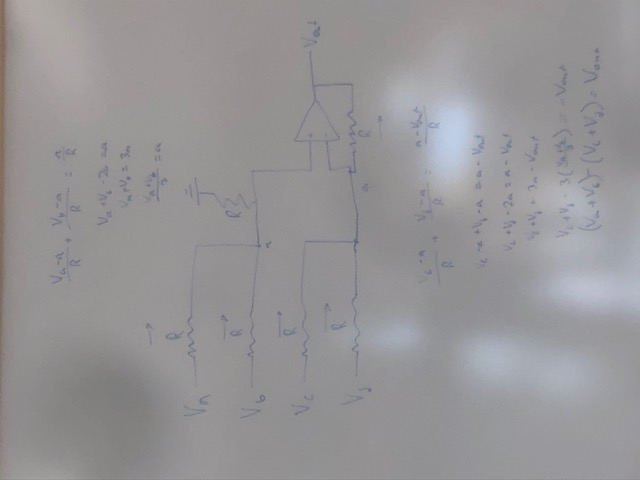
\includegraphics[angle=270,scale=.75]{1.jpg} \end{center}

    Thus, $(\text{V}_a + \text{V}_b) - (\text{V}_c + \text{V}_d) = \text{V}_{\text{out}}$.

\newpage\noindent\textbf{7.}

    With positive Vin, the diode will conduct, so Vout = Vin, as expected (assuming an ideal diode)
    With negative Vin, the diode will not conduct, so Vout = 0.
    Thus, when Vin is a 0.2V amplitude sinewave at 100Hz, Vout would look like this:
    \begin{center}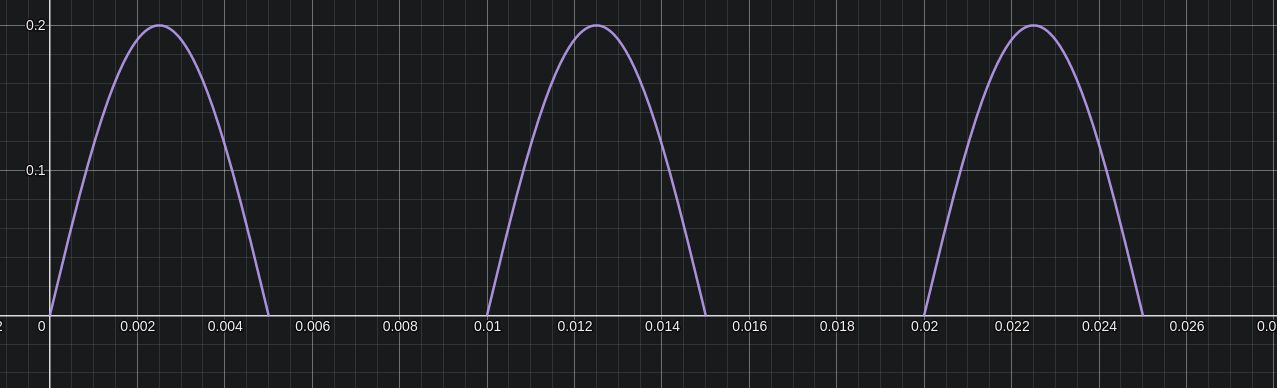
\includegraphics[scale=.5]{3.png}\end{center}
    
\newpage\noindent\textbf{8.}

    \begin{center} 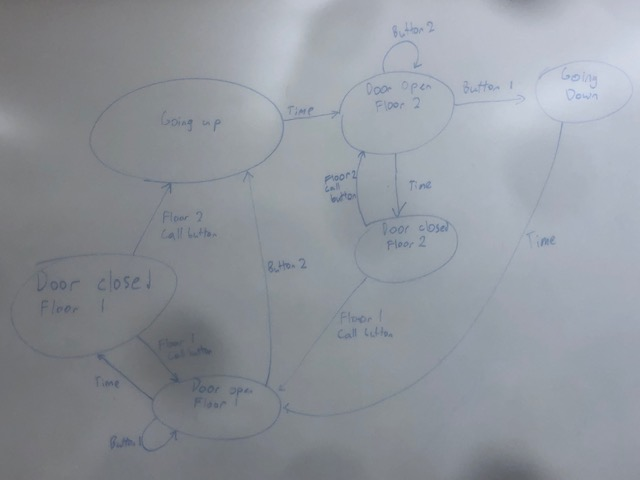
\includegraphics[scale=.7]{4.jpg} \end{center}

\end{document}
